\chapter{Model Selection and Training}
\minitoc
\newpage

\setcounter{secnumdepth}{0} % Set the section counter to 0 so next section is not counted in toc
% ----------------------- Introduction ----------------------- %
\section{Introduction}
In what follows, we will discuss the model selection and training process.
We will start by splitting the data into training and testing sets.
Then, we will train the model on the training set and evaluate it on the testing set.
Finally, we will interpret the results and discuss how the model can be used.

\setcounter{secnumdepth}{2} % Resume counting the <sections for the toc with a depth of 2 (Sections and sub-sections)
% ----------------------------------- SECTIONS (v) ----------------------------------- %
% ----------------------- Model Selection ----------------------- %
\section{Model Selection}

\subsection{Recommendation System Overview}

\cite{nvidia} A recommendation system (or recommender system) is a class of machine learning that uses data to help predict, narrow down, and find what people are looking for among an exponentially growing number of options.

Recommendation systems are used by pretty much every major company in order to enhance the quality of their services and products.

For example, Netflix uses recommendation systems to suggest movies and TV shows to its users, Amazon uses them to suggest products, and Spotify uses them to suggest music.

\begin{figure}[H]
    \centering
    \makebox[\textwidth]{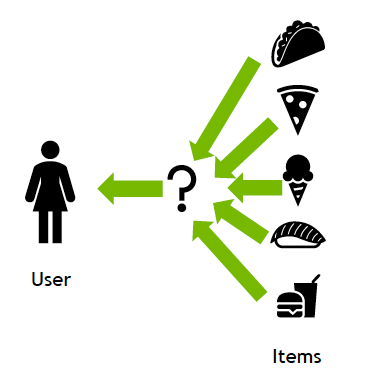
\includegraphics[width=8cm]{src/assets/images/recommendation-system.png}}
    \caption{Recommendation System Sketch}
    \label{fig:recommendation-system-sketch}
\end{figure}

\subsection{Considered Algorithms}

Recommendation systems are usually classified into two categories: content-based and collaborative filtering.

There are also hybrid recommendation systems that combine both approaches, but in this report, we will only focus on the two main categories.

\subsubsection*{Content-Based Filtering}

Content filtering leverages the characteristics or attributes of an item (hence the term 'content') to suggest other items that align with the user's preferences.

Let's look at an example from NVIDIA \cite{nvidia}:

\begin{figure}[H]
    \centering
    \makebox[\textwidth]{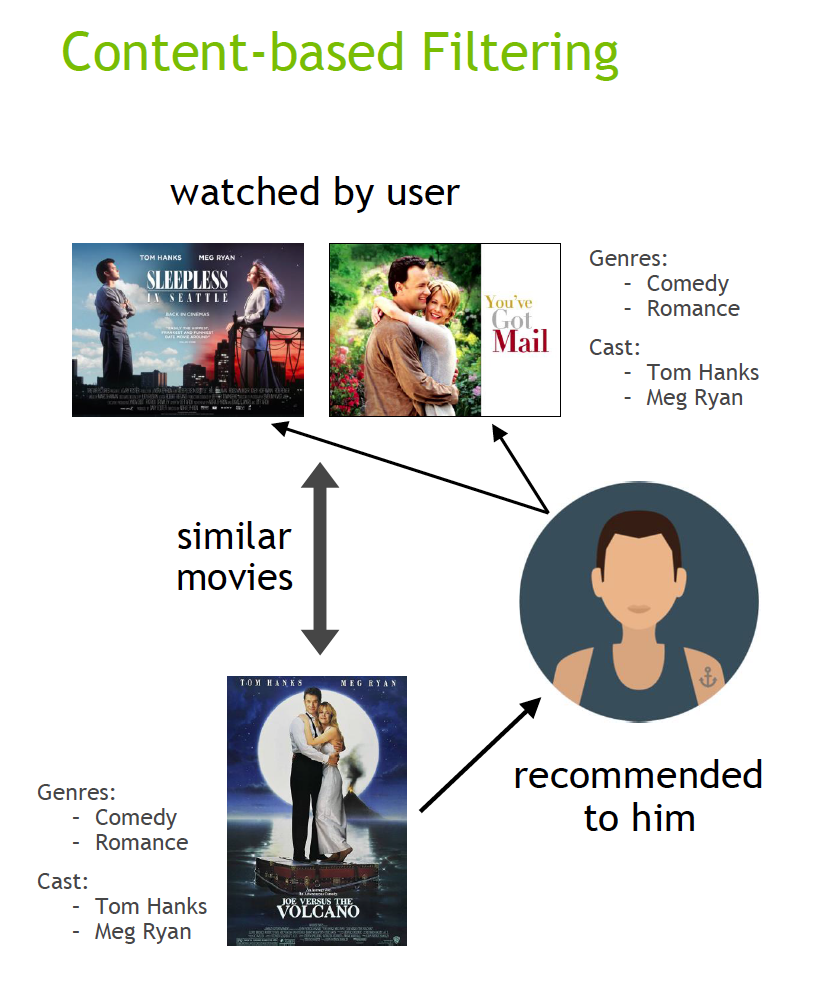
\includegraphics[width=8cm]{src/assets/images/content-based-filtering.png}}
    \caption{Content-Based Filtering Example}
    \label{fig:content-based-filtering-example}
\end{figure}

If a content filtering recommender sees you liked the movies You've Got Mail and Sleepless in Seattle, it might recommend another movie to you with the same genres and/or cast such as Joe Versus the Volcano.

\subsubsection*{Collaborative Filtering}

Collaborative filtering -by contrast- recommends items (filtering) based on the preferences of other users (collaborating).
This approach is based on similarity of item and user features,  given information about a user and items they have interacted with (e.g. a user's age, the category of a restaurant's cuisine, the average review for a movie),  model the likelihood of a new interaction.

The idea is that if some people have made similar decisions and purchases in the past, like a movie choice, then there is a high probability they will agree on additional future selections.

Looking at yet another example from NVIDIA \cite{nvidia}:

\begin{figure}[H]
    \centering
    \makebox[\textwidth]{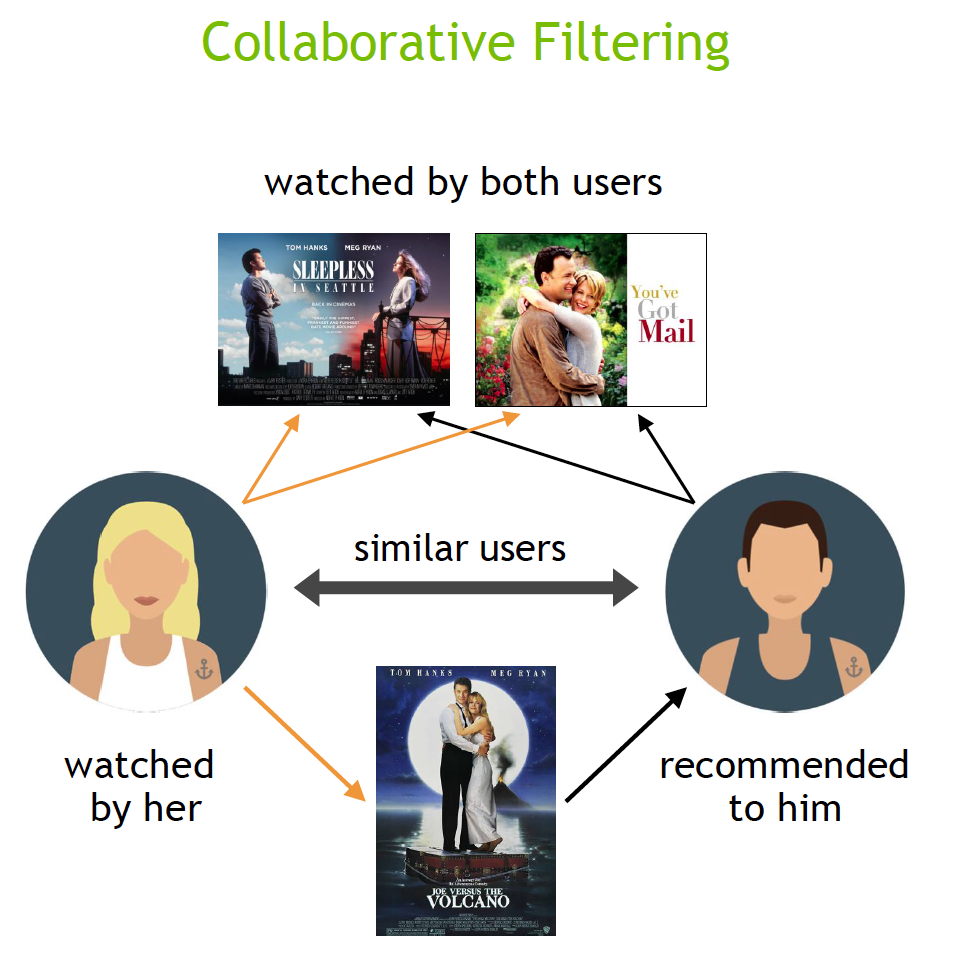
\includegraphics[width=8cm]{src/assets/images/collaborative-filtering.png}}
    \caption{Collaborative Filtering Example}
    \label{fig:collaborative-filtering-example}
\end{figure}

This is the algorithm that we will be using in this project.

% ----------------------- Data Splitting ----------------------- %
\section{Data Splitting}

\subsection{Train-Test Split}
In order to evaluate our recommendation model effectively, we split our data into a training set and a test set.
The training set is used to train the model, while the test set is used to evaluate its performance on unseen data.

We stick to the common 80-20 split, where 80\% of the data is used for training and 20\% is used for testing.

\subsection{Normalization/Scaling}
Before training a model, the data needs to be scaled to ensure the the model learns more effectively and prevents features with larger scales from dominating the learning process.

In our case, this is partially done during the preprocessing pipeline and will be completed during the training process.

% --------------- Model Training --------------- %
\section{Model Training}

\subsection{Algorithm implementation}
Since we will be using collaborative filtering -which is an unsupervised learning algorithm- we will using `TruncatedSVD' from the scikit-learn library.

`TruncatedSVD` stands for Truncated Singular Value Decomposition.
It is a dimensionality reduction technique.

In the context of recommendation systems (such as the case here), `TruncatedSVD` is used to discover latent features in the user-item matrix. The aformentioned latent features are used to make recommendations.

\subsection{Training Process}
During the training process, the model should learn to predict which messages are most likely to make a lead convert based on the features of the leads and the messages they have interacted with in the past.

% --------------- Model Evaluation & Validation --------------- %
\section{Model Evaluation \& Validation}

\subsection{Evaluation Metrics}
Several metrics can be used to evaluate the performance of a recommendation system.
In this case, the best number of dimensions is the one that captures the most information, as measured by the explained variance ration.

\subsection{Validation Strategy}
In order to evaluate the model's performance, we will use the test set that we created earlier.
But first, we will be doing some hyperparameter tuning to find the best number of dimensions.

The goal is to find the optimal number of components `n\_components`that maximizes the explained variance ratio, which is a measure of how much information (variance) can be attributed to each of the principal components.

% --------------- Interpretation --------------- %
\section{Interpretation}

\subsection{Feature Importance}
By analyzing the feature importance, we can gain insights into which features are most influential in the model's predictions. This can help us understand why certain messages are more effective than others.

The features of particular importance to us are:
\begin{itemize}
    \item \textbf{n\_components}: These are the latent features derived from the user-item matrix, capturing the underlying patterns in the data. In our context, they represent specific interaction patterns between leads and messages.
    \item \textbf{Explained Variance Ratio}: This metric indicates the proportion of the data's variance that can be explained by the latent features. Essentially, it quantifies the amount of information captured by these features.
\end{itemize}

\subsection{Model Explanation}
The created latent features do not directly correspond to the original features in the data. The transformed user-item matrix can be used to see how each lead is represented in terms of latent features.

% --------------- Using the Model --------------- %
\section{Using the Model}
The model can be used to predict which messages are most likely to make a lead convert.
This can be done by using specific model methods.
Furthermore, to make the model more accessible and easy to use, it can be exported and then integrated into a web service.
This allows users to make predictions directly via API calls, enhancing the usability and practicality.
This will be entailed in the next chapter.

% ----------------------------------- SECTIONS (^) ----------------------------------- %

\setcounter{secnumdepth}{0} % Set the section counter to 0 so next section is not counted in toc
% ----------------------- Conclusion ----------------------- %
\section{Conclusion}
In this chapter, we discussed the model selection and training process.
We then moved to evaluating and validating the model, then we concluded by interpreting the results and hinting at how the model can be used.
In what follows, we will talk about the latest chapter of the project: the realization.
